\section{JAVA and Benchmarking Pitfalls}

In this section, some of the important points to take care of in
micro-benchmarking with JAVA are presented. The implementation of our benchmark
platform is based on the technical advices from \cite{boyer:2008:bench}, where
more details about the technical aspects can be found.

\begin{description}
\item[Time recording] With micro-benchmarking, the running time is generally
below 10 ms. Thus using the method \#System.currentTimeMillis() is not adapted.
An other method for recording such short running times is available within that
same class, \#System.nanoTime(), which gives a time at the nano-second precision.
\item[Warm up] The JVM works on the code while it is being run. Indeed the JVM
is based on just-in-time (JIT) compilation, thus the JVM performs some
optimizations on the code at runtime, thanks to various statistics gathered. In
order to decrease the noise because of those heuristics, the portion of code
being evaluated has to be run several times, without any measures being
recorded. In doing so, the classes that are used during the benchmark are
already ``loaded'' by the JVM. \cite{boyer:2008:bench} reports that doing so for
10 seconds is enough to have most of the JVM optimizations done.
\item[Dynamic optimization] Even though the warm up phase decreases the number
of optimizations likely to be done by the JVM hereafter, it is still possible
that some are executed while measuring the running time. In order to detect
these changing state of the JVM, we can use the JAVA classes
\emph{ClassLoadingMXBean} and \emph{CompilationMXBean} within the package
``java.lang.management'' that reports various statistics about the JVM, e.g. the
number of loaded classes.

On line 2 and 3, we instantiate objects that gives information about the state
of the JVM. ClassLoadingMXBean reports the number of classes that have been
loaded/unloaded since the JVM started. CompilationMXBean reports the time
ins ms spent on compilation. By wrapping the evaluated code with such
recordings of the JVM (lines 5 to 7 and 13 to 15), we are able to detect that
the JVM performed an optimization by testing those variables: if they are
different, the JVM state changed and so the evaluation need to be restarted.
This allows to make sure that the evaluated time returned is as ``clean'' as
possible.
\lstset{basicstyle=\small,language=Java,commentstyle=\color{red},
emph={ClassLoadingMXBean,CompilationMXBean},emphstyle=\color{blue}}
\begin{lstlisting}[frame=single,numbers=left]
// MF is the namespace used for ManagementFactory
ClassLoadingMXBean loadBean = MF.getClassLoadingMXBean();
CompilationMXBean compBean = MF.getCompilationMXBean();

long loadedClasses1 = loadBean.getTotalLoadedClassCount();
long unloadedClasses1 = loadBean.getUnloadedClassCount();
long compiledTime1 = compBean.getTotalCompilationTime();

long t1 = System.nanoTime();
// Evaluated Code
long t2 = System.nanoTime();

long loadedClasses2 = loadBean.getTotalLoadedClassCount();
long unloadedClasses1 = loadBean.getUnloadedClassCount();
long compiledTime2 = compBean.getTotalCompilationTime();
\end{lstlisting}
\item[Memory management] The memory usage of an application is managed by the
JVM through the use of two mechanisms that are automatically executed. The user
as no control over them and can occur any time the JVM deems necessary.
\begin{enumerate}
  \item {\bfseries Garbage Collection:} free the allocated memory by objects
  that are no more used. It can be explicitly called by \emph{\#System.gc()}.
  \item {\bfseries Object Finalization:} any objects possess the
  \#finalize() method, which frees all resources used by this object. This
  method is called by the garbage collection mechanism. However it is possible
  to explicitly run this method for all objects which destruction is pending by
  calling the method \emph{\#System.runFinalization()}.
\end{enumerate}
The time spent on running those two mechanisms is an other source of noise in
the benchmark. This can be prevented to some point by calling the \#System.gc()
and \#System.runFinalization() methods until the memory usage stabilizes.

The loop from line 11 to 24 tries to free by force with calls to the previous
presented methods. The loop is repeated until the consumed memory stabilizes
and that the number of objects that are waiting to be destroyed are no more.

\lstset{basicstyle=\small,language=Java,commentstyle=\color{red},
emph={gc,runFinalization},emphstyle=\color{blue}}
\begin{lstlisting}[frame=single,numbers=left]
// Return the amount of memory currently used
long usedMem() {
  final Runtime rt = Runtime.getRuntime();
  return rt.totalMemory() - rt.freeMemory();
}
   
final MemoryMXBean mem = ManagementFactory.getMemoryMXBean();
long usedMemPrev = usedMem();

// Upper bound of 100 iterations in order to prevent an ininite loop
for (int i = 0; i < 100; i++) {
  // Trying to free memory 
  System.runFinalization();
  System.gc();

  final long usedMem Now = usedMem();
  // Return the number of objects waiting for finalization
  final int county = mem.getObjectPendingFinalizationCount();

  if ((oCount == 0) && (usedMemNow >= usedMemPrev)) // Memory usage stable
    break;
  else
    usedMemPrev = usedMemNow;
}
\end{lstlisting}
\end{description}

\section{Experimental Environment}

In this section is presented the benchmarking framework that is used for all
benchmarks results presented in the next chapters.

\paragraph{Experimental Settings}

The hardware system we use in our experiments is a 2 x Opteron 250 @ 2.4 GHz
(2 cores, 1024 KB of cache size each) with 4GB memory and a local 7200 RPM
SATA disk. The operating system is a 64-bit Linux 2.6.31-20-server. The
version of the Java Virtual Machine (JVM) used during our benchmarks is
1.6.0\_20. The compression algorithms and the benchmark platform are written
in Java and based on the open-source project Apache Lucene\footnote{Apache
Lucene: \url{http://lucene.apache.org/}}.

\paragraph{Experimental Design}

The benchmarking design below takes into consideration the different critical
points that were previously presented. Each evaluation of the benchmark where
made by
\begin{quote}
\begin{enumerate}
  \item[Initialisation of the benchmark environment]
  \item flushing the OS cache;
  \item initialising a new JVM; 
  \item warming the JVM by executing a certain number of times the benchmark
  until 10 seconds is reached.

  \item[Evaluation of the benchmarked code]
  \item Each measurement is made by performing $n$ times the evaluated code
  execution, with $n$ chosen so that the runtime is long enough to minimise the
  time precision error of the OS and machine (which can be 1 to 10
  milliseconds) to a maximum of 1\%. The measurement time is the CPU time,
  i.e., user time and system time, used by the current thread.
  \item the previous step is re-run if the JVM state changed.
  \item the average running time is recorded.

  \item steps from 4 to 6 are repeated 100 times.
  \item[] As recommended in \cite{lilja:2000:book}, we report the harmonic mean
  and the standard deviation of the 100 measurements.
\end{enumerate}
\end{quote}
The JVM warmup is necessary in order to be sure that the OS and the JVM have
reached a steady state of performance, e.g., that the critical portion of code
is JIT compiled by the JVM.

\subsection{Measurements}

The benchmark produces 100 measurements for one evaluation so that an average
running time can be given, with its standard deviation. However one has to be
wary regarding such results. Indeed while the standard deviation allows to have
a better critic about the running time, it can also lead to misinterpretations.

The \emph{Vysochansk\"i-Petunin} inequality shows that 95\% of the measurements
lie within an interval of three times the standard deviation around the mean.
When comparing two different evaluations with these statistics, one cannot say
which one is faster if that interval around the mean overlaps. The
Figure~\ref{fig:non-overlapping-means} depicts the case where two evaluations
have their intervals non-overlapping, in which case it is possible to say that
the evaluation with the lower mean is better. However this is not the case if
intervals do overlap, as it is the case in the
Figure~\ref{fig:overlapping-means}. Indeed we can have a measurement belonging
to evaluation 2 faster than one from the evaluation 1, even though the mean of
evaluation 1 is lower than the mean of evaluation 2. In such a case, we cannot
say which one is faster, only that the two evaluated codes are similar.

\begin{figure}
\resizebox{\linewidth}{!}{%
\subfloat[Non-overlapping standard deviations.]{%
\centering
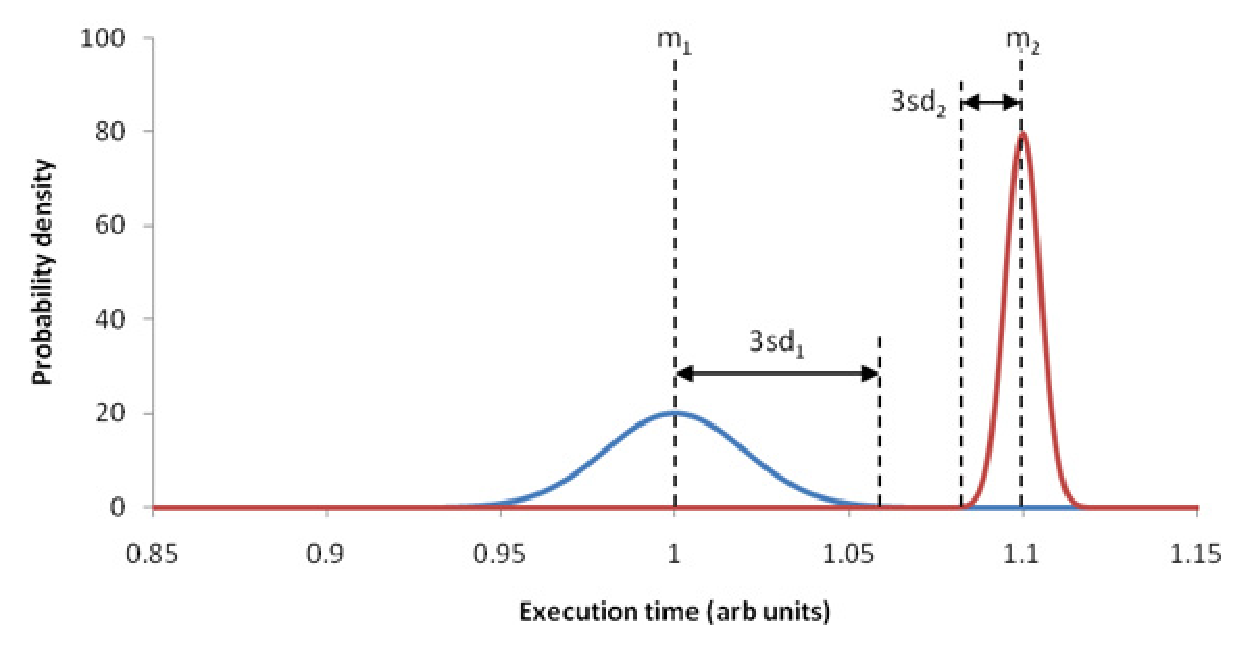
\includegraphics[scale=0.47]{pics/non-overlaping-means}
\label{fig:non-overlapping-means}
}\quad
\subfloat[Overlapping standard deviations.]{%
\centering
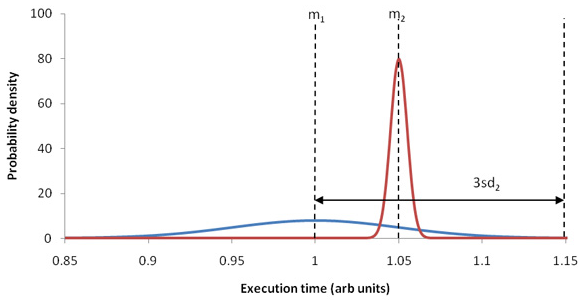
\includegraphics[scale=0.47]{pics/overlaping-means}
\label{fig:overlapping-means}
}}%
\caption{Benchmarks results of two measurements reported with means ($m_i$) and
standard deviations ($sd_i$).}
\end{figure}

% Since the conclusions that we can drawn from the results are based on the mean
% and the standard deviations values, we need to know how much reliability we can
% put into them. Because of all the points that have to be taken care of while
% benchmarking, it is not impossible that some noise still persists while the
% evaluation. With the set of 100 measurements, there are two techniques that can
% inform on the reliability aspect of the statistics, \emph{confidence
% intervals}~\cite{boyer:2008:bench} and the \emph{ANOVA}~\cite{lilja:2000:book} method.
% \begin{description}
% \item[confidence intervals] Means and standard deviations are single computed
% value (i.e. a point estimate), and another run of the benchmark might output
% other results for some reason (e.g. maintenance operations by the system,
% outside of a user control). On the opposite, confidence intervals give a range
% of estimates. A probability p called the confidence level is associated with
% this range. Most commonly, p is chosen to be 95\% and is kept constant during
% confidence interval comparisons. Confidence intervals are intuitive because
% their size indicates reliability: short intervals indicate that the statistic
% is precisely known, while wide intervals indicate uncertainty. For example, if
% the confidence interval for the mean execution of task A is [1, 1.1]
% milliseconds, and that for task B is [0.998, 0.999] milliseconds, then B's
% mean is known with more certainty than A's and is also distinguishably smaller
% (at the same confidence level).
% Confidence intervals can be computed thanks to the
% \emph{bootstrapping}\footnote{Boostrapping:
% \url{http://en.wikipedia.org/wiki/Bootstrapping_(statistics)}} technique, that
% can work for any statistics. A precise explanation of this technique is outside
% the scope of this report.
% \item[ANOVA] Given a set of algorithms to be evaluated, we run them on our
% benchmark and compute for each algorithm a set of 100 measurements. As depicted
% in the Figure~\ref{fig:overlapping-means}, we cannot state with certainty that
% an algorithm A is better than an algorithm B if their interval given by the
% \emph{Vysochansk\"i-Petunin} inequality overlaps. Moreover the difference
% between two algorithms in the other case might not be real if there was some
% noise. \emph{Analysis of the Variance} is a statistical method that tells at
% some confidence degree if one evaluation is statistically better than an other
% one. Thus we can state clearly that an algorithm A is statiscally faster than an
% algorithm B, meaning that the difference observed between the two are real and
% not the consequence of some noise while benchmarking. 
% \end{description}
% ANOVA makes the assumption that measures noises are independent from one
% evaluation to another and that they follow a Gaussian law, while confidence
% intervals does not make any assumptions about the underlaying data.
